%%%%%%%%%%%%%%%%%%%%%%%%%%%%%%%%%%%%%%%%%%%%%%%%%%%%%%%%%%%%%%%%%%%%%%%%%%%%%%%%%%%%%%%%%
% This is a LaTeX template for Bachelor or Master theses at ZHAW, in accordance with the 
% guidelines provided here:
% https://www.zhaw.ch/en/lsfm/study/studiweb/master-ls/masters-thesis/
%
%
% This template is based on previous works by:
% Steve Gunn (http://users.ecs.soton.ac.uk/srg/softwaretools/document/templates/)
% Sunil Patel (http://www.sunilpatel.co.uk/thesis-template/)
% Matteo Delucchi (https://github.com/matteodelucchi/ZHAW_thesis-template)
%
% University specific kpsewhich geometry.stykpsewhich geometry.stykpsewhich geometry.stychanges were made by:
% Matteo Delucchi
% Norman Juchler
% 
% Template license:
% CC BY-NC-SA 3.0 (http://creativecommons.org/licenses/by-nc-sa/3.0/)
%%%%%%%%%%%%%%%%%%%%%%%%%%%%%%%%%%%%%%%%%%%%%%%%%%%%%%%%%%%%%%%%%%%%%%%%%%%%%%%%%%%%%%%%%

%----------------------------------------------------------------------------------------
% DOCUMENT SPECIFICATION
%----------------------------------------------------------------------------------------
\documentclass[
    11pt,                      % Default font size
    %oneside,                  % One-side binding. Default: Two-side binding / alternating margins
    english,                   % Language. Use ngerman for German (Neue Rechtschreibung)
    singlespacing,             % Spacing option: singlespacing, onehalfspacing or doublespacing
    %nolistspacing,            % Set spacing in lists to single
    %draft,                    % Enable draft mode: no pictures, no links, overfull hboxes indicated
    liststotoc,               % Include list of figures/tables/etc in the table of contents
    %toctotoc,                 % Include the main table of contents to the table of contents
    parskip,                  % Add vertical space between paragraphs
    %nohyperref,               % Disable links in the entire document
    headsepline,               % Show a horizontal line under the header
    %chapterinoneline,         % Place the chapter title and chapter number on one line
    consistentlayout,          % Have the same layout for special chapters: 
                               % declaration, abstract and acknowledgements
]{MastersDoctoralThesis}

% Uncomment the following lines to only include a subset of chapters.
% This is useful for long documents, as typesetting takes a bit of time
%\includeonly{
%    Front/titlepage,
%    Front/imprint,
%    Front/abstract,
%    %Front/declaration,
%    %Front/acknowledgements,
%    %Front/symbols,
%    Chapters/Chapter1,
%    %Chapters/Chapter2
%    }


%----------------------------------------------------------------------------------------
% PREAMBLE: PACKAGES AND CONFIGURATIONS
%----------------------------------------------------------------------------------------
\input{preamble}


%----------------------------------------------------------------------------------------
% THESIS INFORMATION: MODIFY THIS SECTION!
%----------------------------------------------------------------------------------------

% The information below is used in the following parts:
% - Title page
% - Imprint
% - Abstract / Zusammenfassung
% - Meta information of PDF

\thesistitle{Análisis de matrícula de estudiantes de nivel inicial de Educación Básica Regular del 2020, 2021 y 2022}             % Thesis title,              command: \ttitle
\thesistype{Gestión de Datos}             % Type of thesis (e.g. Master Thesis) \ttype
\thesisdate{\today}                     % Date of submission                  \tdate
\keywords{gravity, physics, disruptive science}
                                        % Keywords for the thesis,            \keywordnames
\author{Alexander Cubas Francia\\Ernesto Igor Laura Mamani\\Grabiela Quispe Ochoa\\Yerimen Antonio Campos Luyo}                  % Your name,                          \authorname
\degree{Master of Science ZFH}          % Degree name,                        \degreename
\studyprogram{Applied Computational Life Sciences, M.Sc.} 
                                        % Study program                       \studyprog
\studyprogramlink{https://www.zhaw.ch/en/lsfm/study/master/applied-computational-life-sciences/}
                                        % Link to study program               \studyproglink

\supervisorA{Oscar Efraín Ramos Ponce}       % Name of supervisor 1,               \supnameA
\supervisorAmail{e=mc2@zhaw.ch}         % Email address of supervisor 1,      \supmailA
\supervisorAweb{https://en.wikipedia.org/wiki/Albert\_Einstein}  %            \supwebA
\supervisorAinfo{                       % Formatted info about supervisor 1:  \supinfoA
    \supnameA\\
    Universidad Peruana de Ciencias Aplicadas\\
    Email: \href{mailto:\supmailA}{\supmailA}\\
    Web: \href{\supwebA}{Link}
}

% Keep empty if there is no supervisor 2: \supervisorB{}
\supervisorB{}              % Name of supervisor 2,               \supnameB
\supervisorBmail{f=am@newton.com}       % Email address of supervisor 2,      \supmailB
\supervisorBweb{https://en.wikipedia.org/wiki/John\_Locke}                  % \supwebB
\supervisorBinfo{                       % Formatted info about supervisor 2:  \supinfoB
    \supnameB\\
    University of Cambridge\\
    Email: \href{mailto:\supmailB}{\supmailB}\\
    Web: \href{\supwebB}{Link}
}

\university{Universidad Peruana de Ciencias Aplicadas}
                                        % University name                     \univname
\universitygerman{Zürcher Hochschule für Angewandte Wissenschaften}
                                        % University, in German               \univnameger
\department{Maestría en Data Science} 
                                        % Department,                         \deptname
%\institute{Mastría en Data Science} 
                                        % Institute,                          \instname
\group{Center of Computational Health} 
                                        % Research group                      \groupname

% Links
\universitylink      {https://www.zhaw.ch/en/university/}                   % \univlink
\universitylinkgerman{https://www.zhaw.ch/de/university/}                   % \univlinkger
\departmentlink      {https://www.zhaw.ch/de/lsfm/}                         % \deptlink
\institutelink       {https://www.zhaw.ch/en/lsfm/institutes-centres/icls/} % \instlink
\grouplink           {https://www.zhaw.ch/en/lsfm/institutes-centres/icls/computational-health/} % \grplink



\AtBeginDocument{
\hypersetup{pdftitle=\ttitle} % Set the PDF's title to your title
\hypersetup{pdfauthor=\authorname} % Set the PDF's author to your name
\hypersetup{pdfkeywords=\keywordnames} % Set the PDF's keywords to your keywords
}

\begin{document}
\frontmatter                  % Roman page numbering for the pre-content pages
\pagestyle{plain}             % Default to the plain heading style until the thesis style 
                              % is called for the body content


%----------------------------------------------------------------------------------------
% TITLE PAGE AND IMPRINT
%----------------------------------------------------------------------------------------
% !TEX root = ../main.tex

%----------------------------------------------------------------------------------------
% TITLE PAGE
%----------------------------------------------------------------------------------------

\newgeometry{margin=1in}
\begin{titlepage}

% Make the title page mostly inert to the parskip-setting.
\setlength{\parskip}{0pt}

\begin{center}

\includegraphics[width=1\textwidth]{Figures/upc_p}

%\ifxetex
    \vspace{0.6cm}
    {\zhawtitlefont\color{zhawblue}\LARGE \univname\par}   % University
    \vspace{0.2cm}
%\else
%    \vspace{0.87cm}
%    {\includegraphics[height=17.9pt]{Figures/zhaw_font_eng_font}\par}
%    \vspace{0.05cm}
%\fi
{\Large  \deptname\par}                      % Department
\vspace{0.2cm}
%{\Large A \instname\par}                                 % Institute
\vspace{3.5cm}                            
\textsc{\Large \ttype}                                 % Thesis type
\vspace{0.2cm}
\HRule 
\vspace{0.4cm}
{\huge \bfseries \ttitle\par}                          % Thesis title
\vspace{0.4cm}  
\HRule
\vspace{1.5cm}

 
\begin{minipage}[t]{0.4\textwidth}
\begin{flushleft} 
    \large
    \emph{Integrantes:}\\
    \authorname
\end{flushleft}
\end{minipage}
\begin{minipage}[t]{0.4\textwidth}
\begin{flushright} 
    \large
    \emph{Profesor:} \\
    \supnameA \\
    \supnameB
\end{flushright}
\end{minipage}
\vspace{2cm}
 
\vfill

{\large
Fecha de entrega\\
28 de Octubre de 2022 \\
\vspace{1.5cm}
%Study program:\\
%\studyprog\\
}
\vfill
\end{center}
\end{titlepage}
\restoregeometry

%\let\cleardoublepage\clearpage
%\include{Front/imprint}


%----------------------------------------------------------------------------------------
% DECLARATION
%----------------------------------------------------------------------------------------
% Comment out this section if the declaration of originality from ZHAW is used.
%\include{Front/declaration}
%\cleardoublepage


%----------------------------------------------------------------------------------------
% ABSTRACT
%----------------------------------------------------------------------------------------
%\include{Front/abstract}


%----------------------------------------------------------------------------------------
% ACKNOWLEDGEMENTS
%----------------------------------------------------------------------------------------
%\include{Front/acknowledgements}


%----------------------------------------------------------------------------------------
% LIST OF CONTENTS/FIGURES/TABLES PAGES
%----------------------------------------------------------------------------------------
% Comment out if any of the following is not needed:
\renewcommand{\contentsname}{Índice}
\renewcommand{\chaptername}{Capítulo}
\renewcommand{\tablename}{Tabla}
\renewcommand{\figurename}{Imagen}

{\hypersetup{hidelinks}\tableofcontents}

%\tableofcontents  % Add main table of contents
%\listoffigures    % Add list of figures
%\listoftables     % Add list of tables


%----------------------------------------------------------------------------------------
% ABBREVIATIONS / SYMBOLS
%----------------------------------------------------------------------------------------
%\include{Front/symbols}


%----------------------------------------------------------------------------------------
% DEDICATION
%----------------------------------------------------------------------------------------
%\dedicatory{For/Dedicated to/To my\ldots} 


%----------------------------------------------------------------------------------------
% THESIS CONTENT - CHAPTERS
%----------------------------------------------------------------------------------------
\mainmatter % Begin numeric (1,2,3...) page numbering
\pagestyle{thesis} % Return the page headers back to the "thesis" style

% Include the chapters of the thesis as separate files from the Chapters folder
% Uncomment the lines as you write the chapters

\chapter{Introducción} % Main chapter title
\label{Chapter1} % For referencing the chapter elsewhere, use \ref{Chapter1} 

%----------------------------------------------------------------------------------------

% Define some commands to keep the formatting separated from the content
% Placing such commands in the preamble is a good idea.
\newcommand{\keyword}[1]{\textbf{#1}}
\newcommand{\tabhead}[1]{\textbf{#1}}
\newcommand{\code}[1]{\texttt{#1}}
\newcommand{\file}[1]{\texttt{\bfseries#1}}
\newcommand{\option}[1]{\texttt{\itshape#1}}

%-

\section{Descripción de la información}

En el presente trabajo se está realizando ...

\section{Datos utilizados}

La información con la que se va a trabajar está conformada por los datos de alumnos de niveles inicial, primaria y secundaria de colegios en todo el Perú, esta información corresponde a los 3 últimos años, el detalle de esta entidad se ve en la tabla Table~\ref{tab:estudiantes}

\begin{table}
\caption{Detalle de los campos de la entidad estudiante}
\label{tab:estudiantes}
\centering
\begin{tabular}{l l l}
\toprule
\tabhead{Columna} & \tabhead{Descripción}\\
\midrule
ID Año & Identificador del año escolar\\
Departamento & Nombre del departamento\\
Provincia & Nombre de la provincia\\
Distrito & Nombre del distrito\\
Centro Poblado & Centro poblado \\
NLongitud IE & Coordenada de la longitud de la IE \\
NLatitud IE & Coordenada de la latitud de la IE\\
DRE & Dirección regional de educación\\
UGEL & Ugel a la que pertenece la IE\\
Cod Mod & NN\\
Anexo & NN\\
Nombre IE & Nombre de la Institución educativa\\
D Gestión & NN\\
Dsc Turno & Descripción del turno\\
Modalidad & Modalidad\\
Nivel Educativo & Nivel en el que se encuentra el estudiante\\
Fecha Matrícula & Fecha de la matrícula\\
ID Persona & Identificador del estudiante\\
Documento Identidad & Documento de identidad\\
Sexo & Sexo del alumno\\
Madre vive & Indicador si la madre vive\\
Padre vive & Indicador si el padre vive\\
Dsc Grado & Descripción del grado\\
Dsc Sección & Descripción de la sección\\
Nacionalidad & Nacionalidad del estudiante\\
Dsc Discapacidad & Descripción de discapacidad\\
Dirección & Dirección del estudiante\\
Lugar & Lugar de la dirección\\
Ubigeo & Ubigeo del estudiante\\
\bottomrule\\
\end{tabular}
\end{table}

\section{Importancia de los datos}

Debido a que la información trabajada proviene del ámbito educativo de níveles básicos, se pueden generar estadísticas para poder evaluar el estado actual educativo, ...
\include{Chapters/Chapter1__}
\chapter{Metodología} % Main chapter title
\label{Chapter2} % For referencing the chapter elsewhere, use \ref{Chapter1} 

\section{Metodología utilizada}

En el presente proyecto se ha utilizado la metología CRISP DM\parencite{CrispBook1}, pero sólo en las etapas iniciales que tienen que ver con el trabajo de los datos. En la imagen~\ref{fig:crispdm} se pueden ver resaltadas las etapas cubiertas.

\begin{figure}[th]
\centering
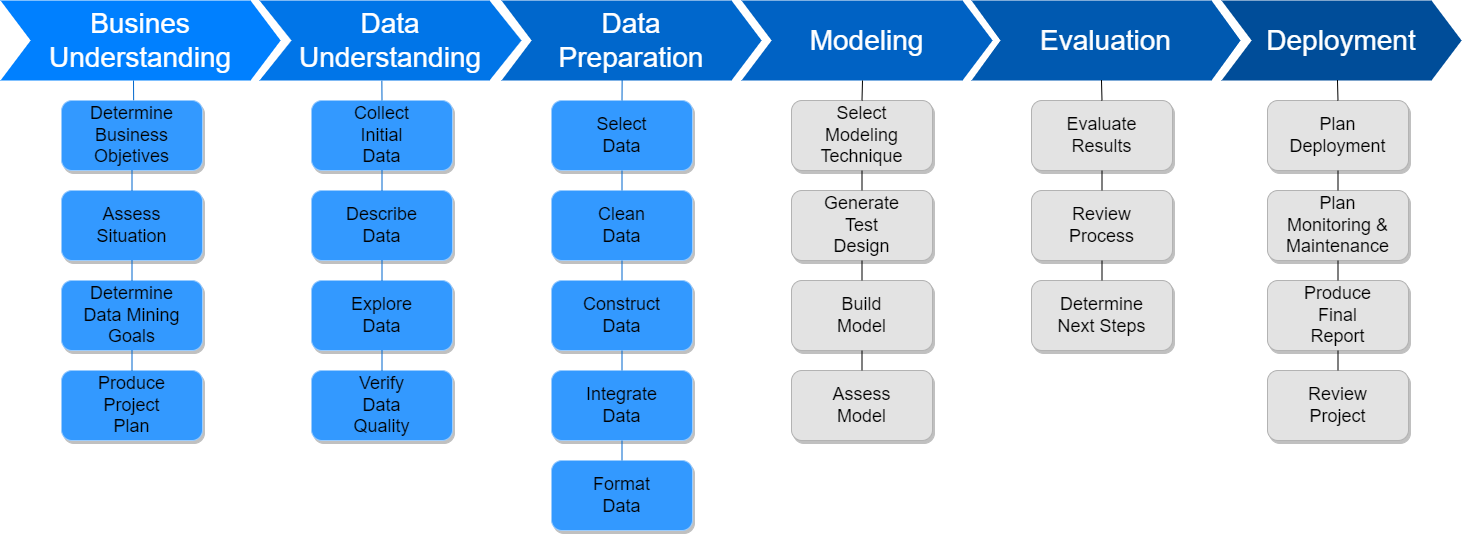
\includegraphics[width=1.2\textwidth]{Figures/modelo_crisp}
\decoRule
\caption[Metodolofía Crisp DM]{Secciones cubiertas en el proyecto}
\label{fig:crispdm}
\end{figure}

\section{Herramientas usadas}

Se han hecho uso de las siguientes herramientas:

\begin{itemize}
\item Base de datos MySql
\item Servicio RDS de AWS
\item R Studio
\item JetBrains DataGrip
\item Shiny
\item Git (github)
\end{itemize}

Se obtuvo un archivo CSV con toda la información de estudiantes, este archivo fue subido mediante DataGrip a una BD MySQL, previamente creada como un servicio RDS de AWS, con estos datos cargados se realizaron procesos mediante R para obtener información que posteriormente fueron registrados en otra base de datos y mostrados mediante una aplicación Shiny.

En la imagen~\ref{fig:proceso} se puede ver el flujo del proceso en este trabajo de análisis.
\begin{figure}[th]
\centering
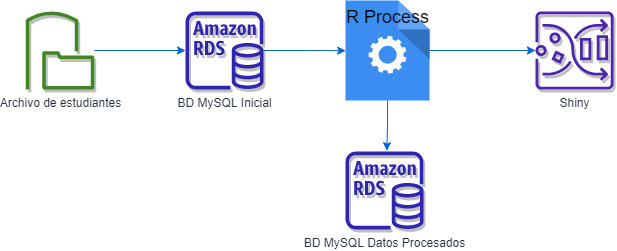
\includegraphics[width=1.1\textwidth]{Figures/proceso-archi}
\decoRule
\caption[Proceso de exploración de los datos]{Herramientas usadas}
\label{fig:proceso}
\end{figure}

\section{Trabajo con los datos}

Para el trabajo con R y MySQL se hizo uso de la bilbioteca RMySQL y DBI, el código para la conexión se encuentra en la sección \ref{codigo_conexionbd}.

\section{Análisis realizados}

\subsection{Niveles educativos}
Para el caso del nivel educativo, es importante conocer la cantidad de alumnos por año en cada nivel, de esta forma identificamos si existe algún incremento o alguna disminución, para lo que se deberá realizar diversas acciones contrarrestando cualquier inconveniente de materiales y de inmobiliarios. \\
En el apéndice \ref{cod_niveles_educativos} está el código fuente de esto.

\subsection{Evolución mensual de matrículas}
\begin{itemize}
\item Se hizo una consulta a la Base de Datos donde se encuentra la tabla estudiante.
\item Debido que sólo había una columna con la fecha de la matrícula en formato YYYY-MM-DD, se obtuvo sólo los valores de año y mes para que se puedan agrupar por este campo.
\item Luego se agrupó esta información por el nuevo campo que contiene el año y el mes.
\item Se categorizó el campo mes.
\item Se agregó un campo de año para que pueda ser filtrado posteriormente.
\end{itemize}

El código para obtener la información para este análisis se encuentra en el anexo \ref{cod_evolucion_matriculas}.

El resultado de este análisis se encuentra en la sección \ref{res_evolucion_matriculas}.

\subsection{Discapacidad}

Para el procesamiento de la data se realizó limpieza de datos vacíos, posterior a eso se agrupó y realizó el conteo de estudiantes que tengan alguna discapacidad.\\
Con estos datos se puede posteriormente filtrar por año para que pueda ser visualizada dinámicamente en shiny. En el apéndice \ref{cod_discapacidad} está el código fuente de esto.

\subsection{Nacionalidades}

Se desea mostrar la cantidad de estudiantes de nacionalidad diferente a la peruana.\\
Para el procesamiento de los datos no se toma en cuenta a los estudiantes con nacionalidad peruana y datos en blanco.\\
En el apéndice \ref{cod_nacionalidades} está el código fuente de esto.

\subsection{Género}

\begin{itemize}
    \item Se analizo la distribución del género de los estudiantes por año, para esto necesitamos todos los DNIs válidos para proceder con el conteo, por lo cual se realizó una limpieza a la data.
    \begin{itemize}
        \item Limpieza a los strings de genero ya que se encontraban con saltos de línea:
        \begin{figure}[th]
        \centering
        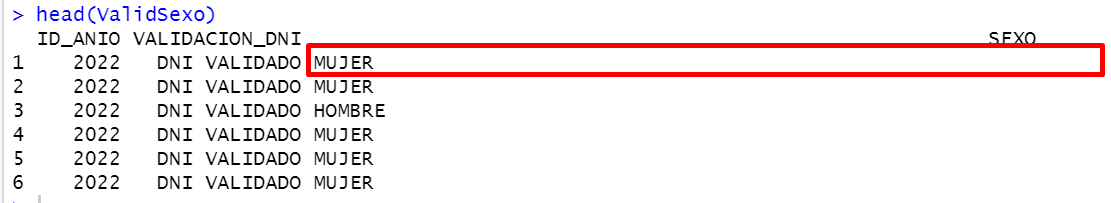
\includegraphics[width=1\textwidth]{Figures/genero1}
        \decoRule
        \caption[]{}
        \label{fig:genero1}
        \end{figure}
        \item Para ello solo extraemos una parte del string (6 primeros caracteres) y está solucionado:
        \begin{figure}[th]
        \centering
        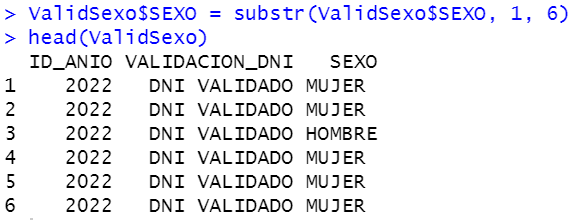
\includegraphics[width=0.6\textwidth]{Figures/genero2}
        \decoRule
        \caption[]{}
        \label{fig:genero2}
        \end{figure}
    \end{itemize}
    \item Se lee la información con un parámetro que quita los registros en blanco, para evitar DNIs que no sean válidos.
\end{itemize}

El código se encuentra en el apéndice \ref{cod_genero}

\subsection{DNI Validados}

\begin{itemize}
    \item Se agrupa el dataframa de estudiantes por el campo de validación de DNI.
    \item Se crea un nuevo DF que contiene el conteo del campo que representa la validación de un DNI.
    \item Se obtiene un porcentaje de los calores del paso anterior.
\end{itemize}

El código se encuentra en el apéndice \ref{cod_dnivalidados}

\section{Uso de shiny}

Se usó Shiny \parencite{ShinyRef} para mostrar los análisis de manera interactiva, ya que se tiene información de 3 años (2020, 2021 y 2022). 

Los componentes utilizados en el proyecto fueron tablas, gráfico de barras, gráfico circular y gráfico de líneas \parencite{RBook1}.
El código para realizar esta funcionalidad se encuentra en el anexo \ref{cod_shiny}.

Para la publicación se hace uso del servidor que brinda RStudio \parencite{ShinyAppRef}.
 
\section{Fuentes}
Las fuentes del proyecto se encuentran en el repositorio Git: \url{https://github.com/Maestria-Data-Science-UPC-G1/gestiondatos.git} 
\chapter{Resultados} % Main chapter title
\label{Chapter3 } % For referencing the chapter elsewhere, use 

\section{Nivel educativo}

Para el caso del nivel educativo, es importante conocer la cantidad de alumnos por año en cada nivel, de esta forma identificamos si existe algún incremento o alguna disminución, para lo que se deberá realizar diversas acciones contrarrestando cualquier inconveniente de materiales y de inmobiliarios. Ver la imagen~\ref{fig:niveleseducativos}

\begin{figure}[h]
\centering
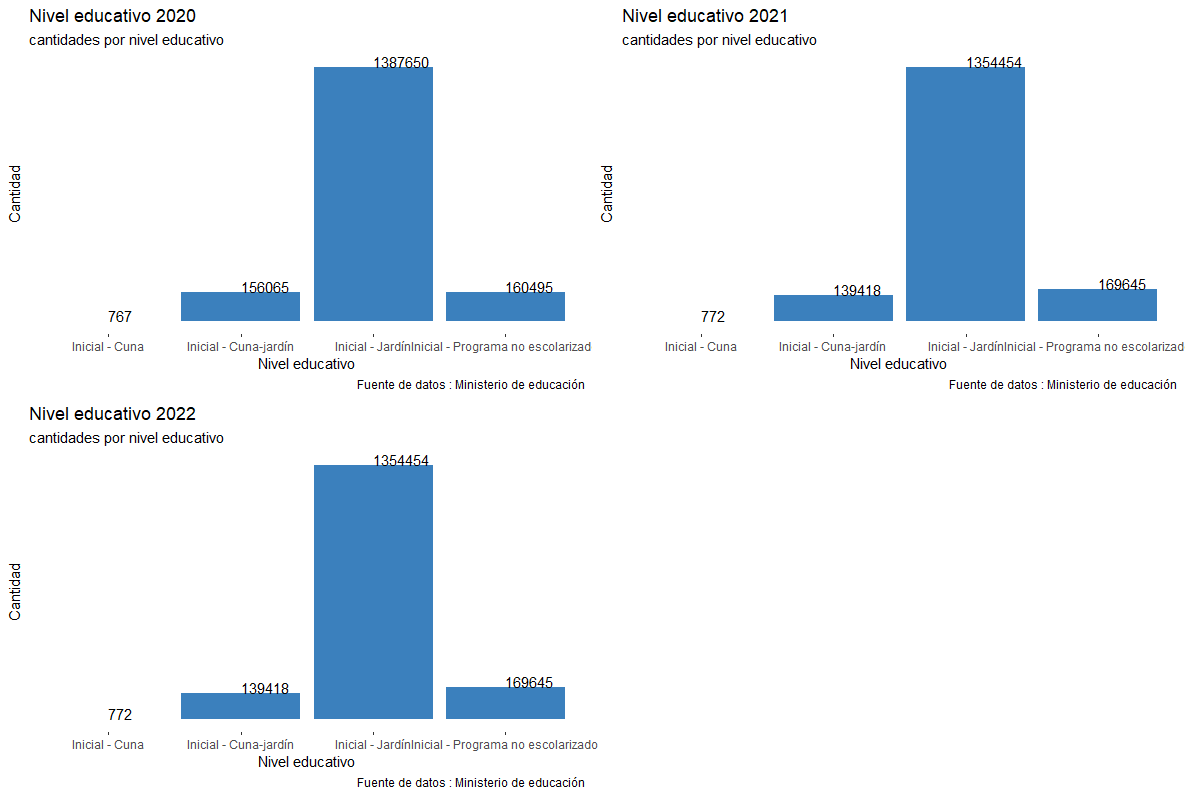
\includegraphics[width=1.2\textwidth]{Figures/nivelesEducativos}
\decoRule
\caption[Nivel Educativo]{Niveles educativos}
\label{fig:niveleseducativos}
\end{figure}

\section{Evolución mensual de matrículas}\label{res_evolucion_matriculas}

En este análisis se identificó la evolución que han tenido la cantidad de matrículas de cada mes en los últimos 3 años, las siguientes imágenes~\ref{fig:matriculas} muestran la evolución por año.\\
Se aprecia una mayor cantidad de incidencias entre Marzo y Abril, esto se puede entender por el inicio del año escolar en el Perú. Y en menor medida hay una cantidad elevada de matrículas desde el inicio de año, durante el resto del año se ve una menor cantidad pero si ocurren, esto podría deberse posiblemente a traslados de colegio.

\begin{figure}[h]
\centering
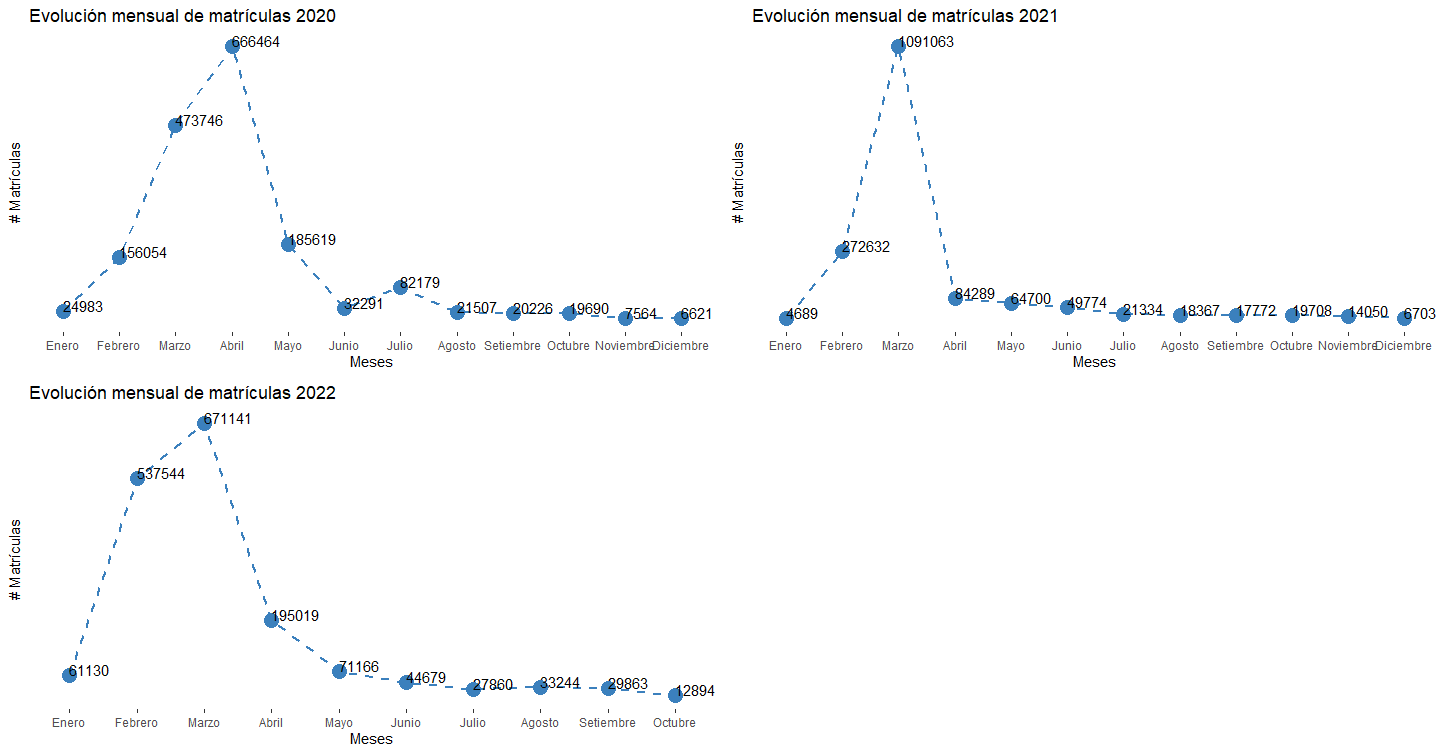
\includegraphics[width=1.2\textwidth]{Figures/evolucionMatriculas}
\decoRule
\caption[Matrículas]{Evolución de cantidades por cada mes}
\label{fig:matriculas}
\end{figure}

\section{Discapacidad}

El presente gráfico~\ref{fig:discapacidad} queremos mostrar la cantidad de estudiantes con alguna discapacidad sea visual, sordoceguera, autismo, auditiva entre otros.\\
Se puede apreciar que en los últimos 2 años se tenía mayor incidencia en las discapacidades motora, intelectual y autismo, pero en el presente año han disminuído las que tienen que ver con motora e intelectual, pero el autismo se mantiene como un factor predominante.

\begin{figure}[th]
\centering
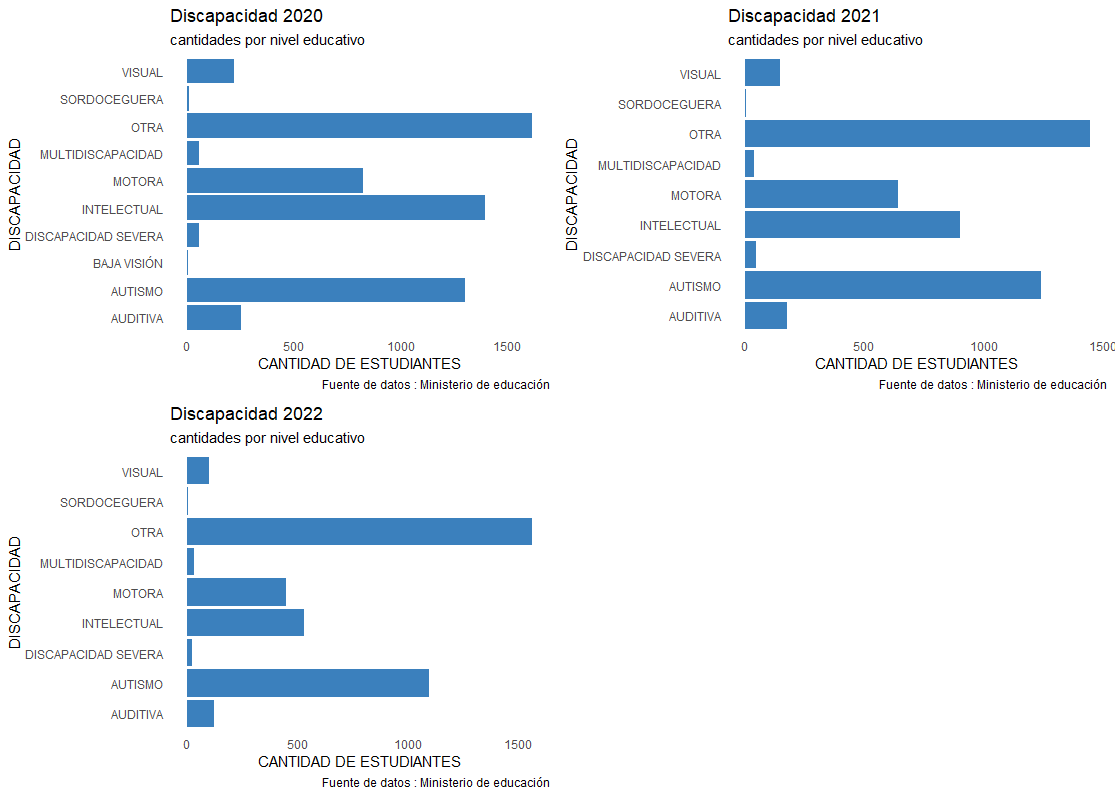
\includegraphics[width=0.8\textwidth]{Figures/discapacidad}
\decoRule
\caption[Discapacidad]{Tipos de discapacidad}
\label{fig:discapacidad}
\end{figure}


\section{Nacionalidad de estudiantes}

Se muestra a continuación una imagen~\ref{fig:nacionalidad} la distribución de nacionalidades, teniendo como mayor cantidad, luego de la peruana, la nacionalidad Venezolana, debido a que hay muchos países en este análisis, se ve conveniente el uso de una tabla para poder mostrar los datos.

\begin{figure}[!h]
\centering
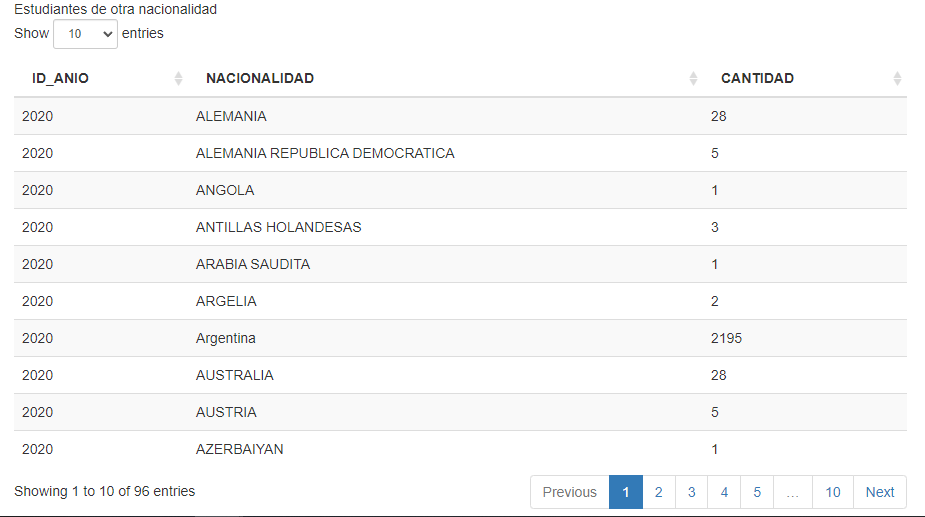
\includegraphics[width=1\textwidth]{Figures/nacionalidad}
\decoRule
\caption[Nacionalidad]{Nacionalidad de estudiantes}
\label{fig:nacionalidad}
\end{figure}

\section{Distribución de género}

En la imagen~\ref{fig:genero} se pueden apreciar distribuciones simulares entre hombres y mujeres.

\begin{figure}[!h]
\centering
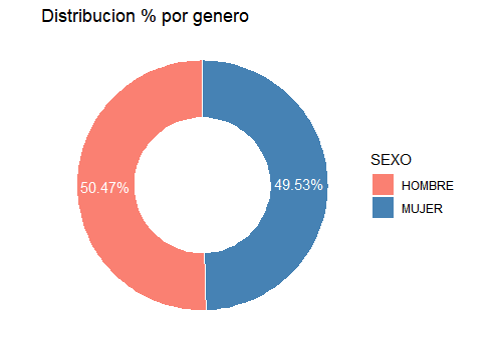
\includegraphics[width=0.8\textwidth]{Figures/genero}
\decoRule
\caption[Genero]{Distribuciones de género}
\label{fig:genero}
\end{figure}

\section{DNI Validados}

En la imagen~\ref{fig:validaciondni} se aprecia que hay una gran mayoría de documentos validados, pero se ve en menor medida estudiantes indocumentados.

\begin{figure}[!h]
\centering
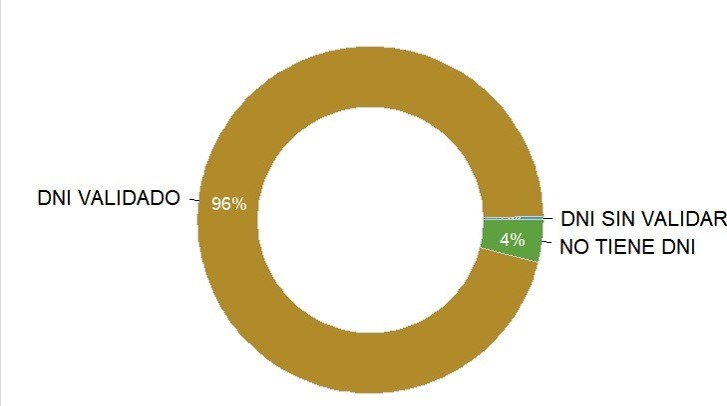
\includegraphics[width=0.8\textwidth]{Figures/validacionDNI}
\decoRule
\caption[DNI Validados]{Validaciones de DNI}
\label{fig:validaciondni}
\end{figure}

\section{Representación por Shiny}
En shiny se desarrolló un panel que tiene un filtro por año para poder filtrar los gráficos presentados anteriormente según la imagen~\ref{fig:shiny}, la reactividad ante este campo de entrada permite tener la visualización de lo que ocurre por año.
\begin{figure}[th]
\centering
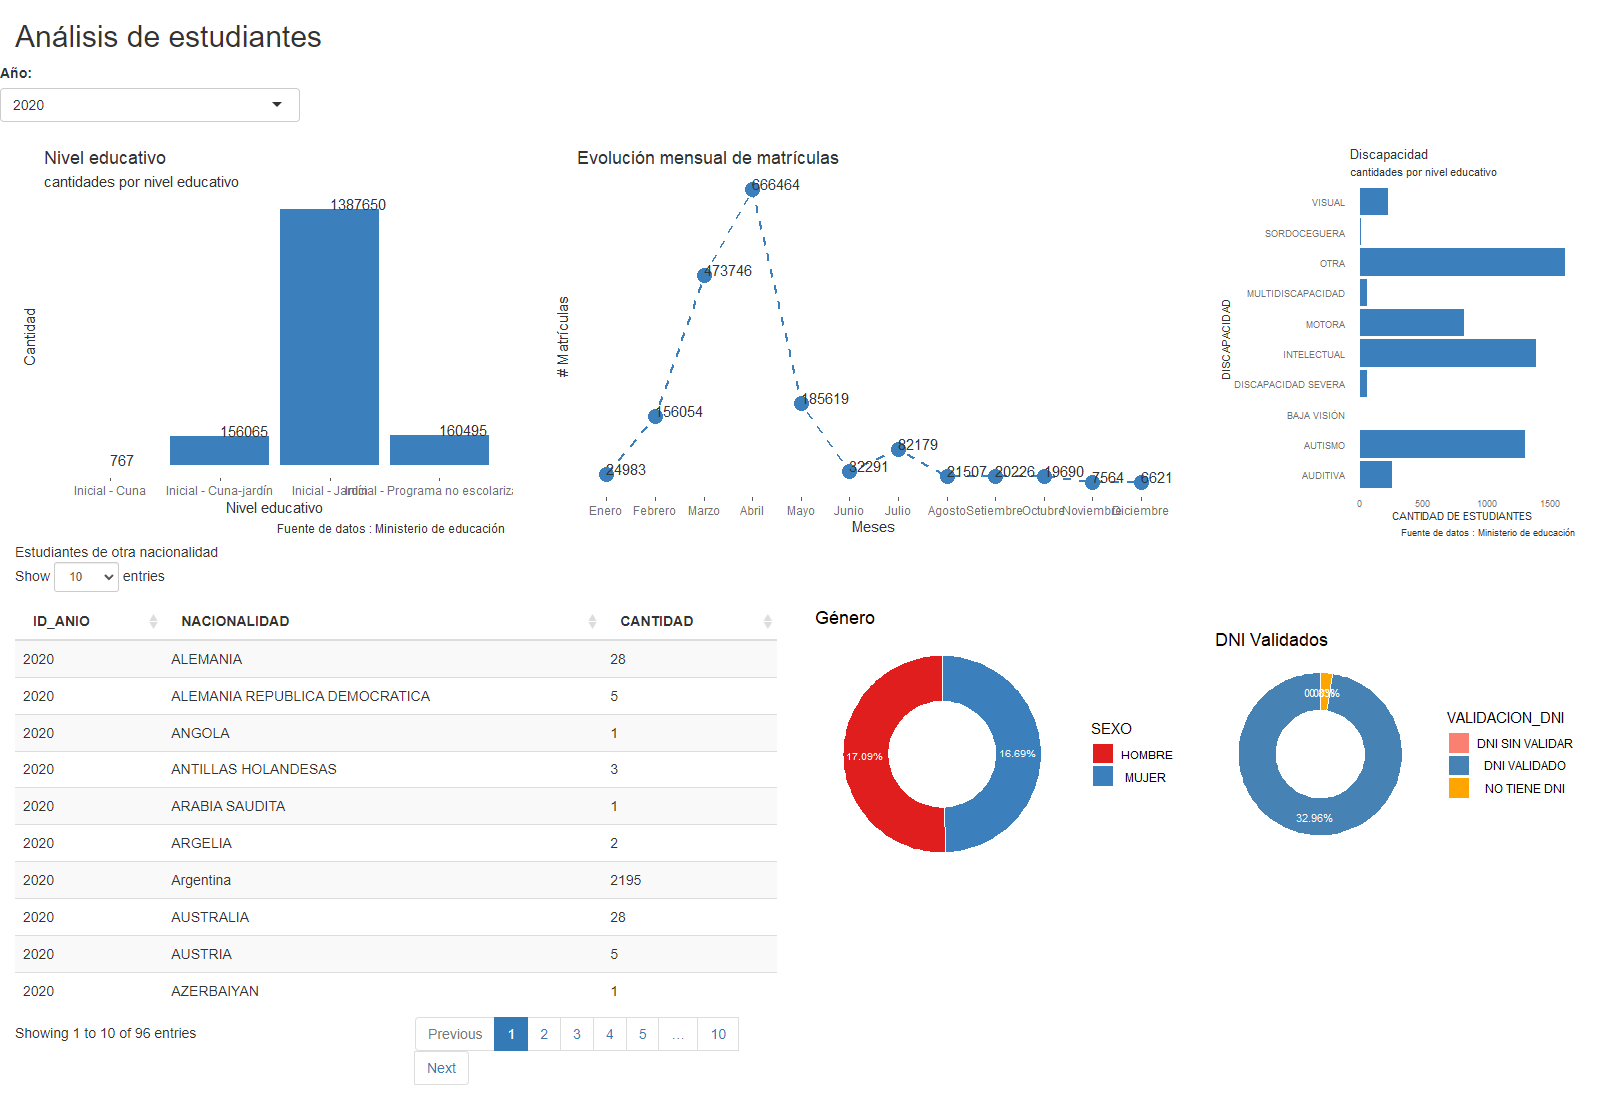
\includegraphics[width=1\textwidth]{Figures/shiny}
\decoRule
\caption[Shiny]{Representación mediante Shiny}
\label{fig:shiny}
\end{figure}

\section{Representaciones de ubicación de instituciones educativas por mapa}

Ya que es importante conocer la ubicación de los colegios, se realizó un mapa utilizando las librerias ggplot2, tidyverse y mapview en R, esta última librería proporciona funciones para crear visualizaciones interactivas de datos espaciales de manera muy rápida y conveniente. El código de estas representaciones se encuentra en el anexo \ref{cod_mapas}

Diagrama~\ref{fig:mapa1}: Su objetivo principal es llenar el vacío del trazado interactivo rápido (sin grado de presentación) para examinar e investigar visualmente ambos aspectos de los datos espaciales, las geometrías y sus atributos

\begin{figure}[th]
\centering
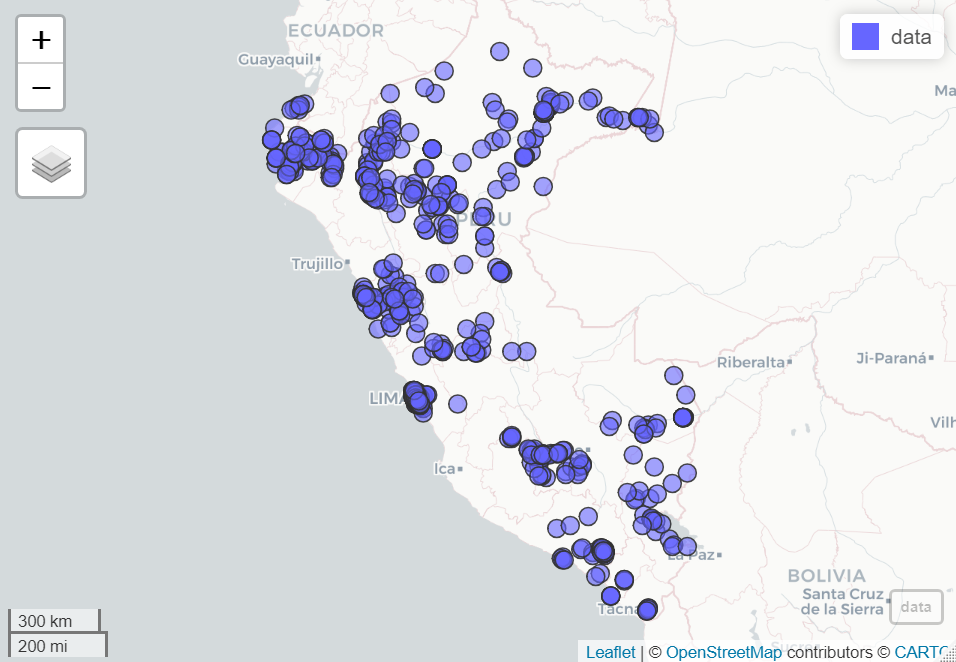
\includegraphics[width=1\textwidth]{Figures/mapa1}
\decoRule
\caption[Mapa]{Representación geográfica}
\label{fig:mapa1}
\end{figure}

Diagrama~\ref{fig:mapa2}: También podemos ver un conteo rápido del número de colegios por sector, con la librería leaflet, con una muestra que se extrajo, podemos ver a medida que vamos aumentando el zoom en que zonas entan mayor concentrados los colegios. 

\begin{figure}[th]
\centering
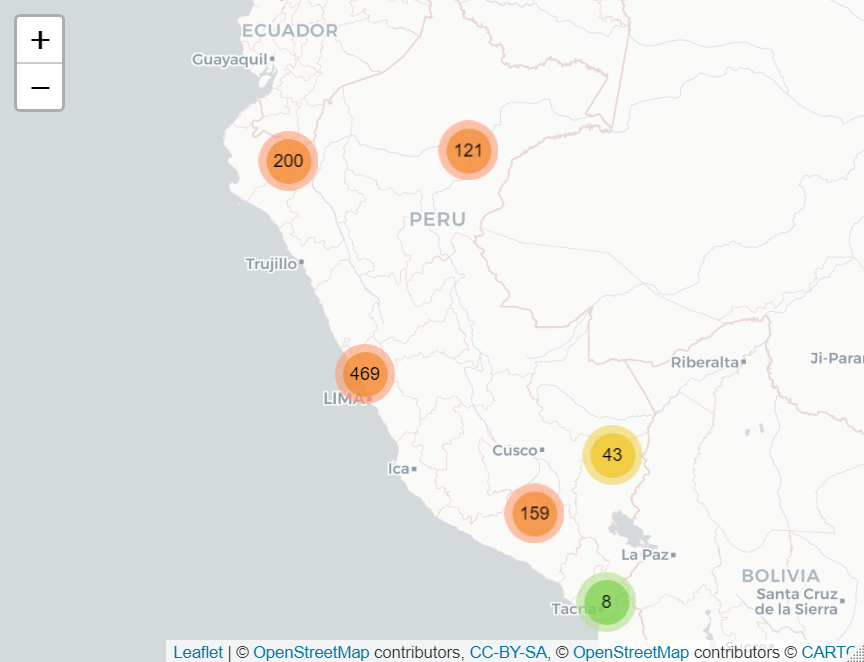
\includegraphics[width=1\textwidth]{Figures/mapa2}
\decoRule
\caption[Mapa]{Colegios}
\label{fig:mapa2}
\end{figure}

Diagrama~\ref{fig:mapa3}:Aprovechamos la interactividad del gráfico y cada que acercamos (zoom) nos muestra la cantidad de colegios acumulados en cada zona.

\begin{figure}[th]
\centering
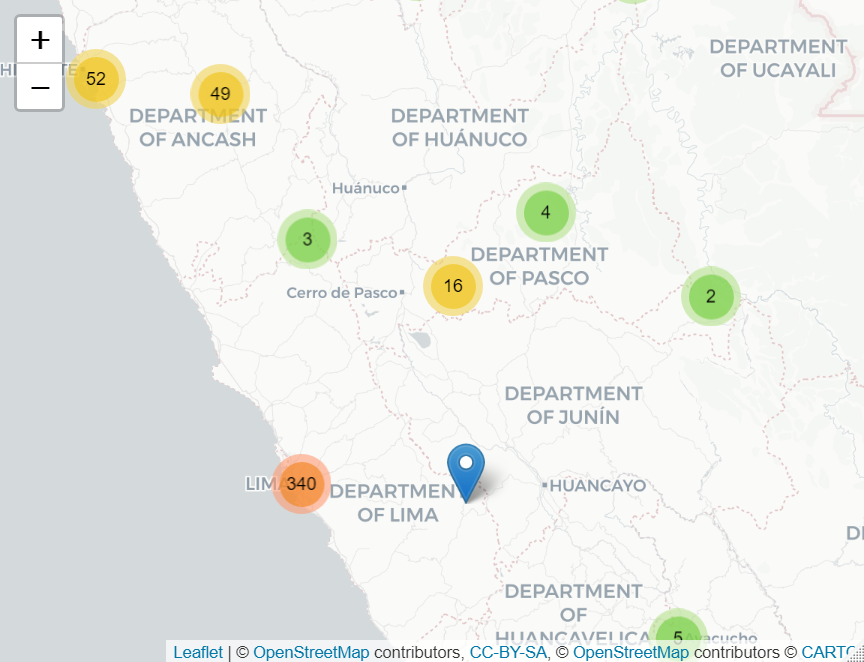
\includegraphics[width=1\textwidth]{Figures/mapa3}
\decoRule
\caption[Mapa]{Instituciones educativas acumuladas}
\label{fig:mapa3}
\end{figure} 
%\include{Chapters/Chapter2_} 
\chapter{Anexos}
\label{Anexos} % For referencing the chapter elsewhere,

 \section{Código de conexión a la base de datos}\label{codigo_conexionbd}
\begin{lstlisting}[language=R]
library(shiny)
library(ggplot2)
library(DBI)
library(RMySQL)
library(reshape2)

id_host = "localhost"
db <- dbConnect(RMySQL::MySQL(),
                dbname = "bd_gestiondatos",
                host = id_host,
                user = "root",
                password = rstudioapi::askForPassword("Database password"),
                Port     = 3306)
\end{lstlisting}

\section{Evolución mensual de matrículas}\label{evolucion_matriculas}
\begin{lstlisting}[language=R]
getMonthDay = function(arrayMes) {
  month = as.Date(arrayMes)
  fec = format(month, "%Y-%m")
}

getFormatedMonth <- function(arrayMes) {
  nombre_meses <- c("01"="Enero", "02"="Febrero", "03"="Marzo",
                    "04"="Abril", "05"="Mayo", "06"="Junio",
                    "07"="Julio", "08"="Agosto", "09"="Setiembre",
                    "10"="Octubre", "11"="Noviembre", "12"="Diciembre")
  mo = nombre_meses[substr(arrayMes, 6, 7)]
}

df <- dbGetQuery(db, 'SELECT * FROM estudiante')
df2 = df

df2$month = getMonthDay(df2$FECHA_MATRICULA)
df2 = data.frame(df2$FECHA_MATRICULA, df2$ID_PERSONA, df2$month)

df_graph = aggregate(x = df2.ID_PERSONA ~ df2.month, 
                     data = df2, 
                     FUN = length)

df_graph$df2.month <- factor(df_graph$df2.month, levels = df_graph$df2.month, ordered=T)

df_graph$formated_month = getFormatedMonth(df_graph$df2.month)
df_graph$anho = substr(df_graph$df2.month, 1, 4)


\end{lstlisting}
%\chapter{Resultados} % Main chapter title
\label{Chapter3 } % For referencing the chapter elsewhere, use 

\section{Nivel educativo}

Para el caso del nivel educativo, es importante conocer la cantidad de alumnos por año en cada nivel, de esta forma identificamos si existe algún incremento o alguna disminución, para lo que se deberá realizar diversas acciones contrarrestando cualquier inconveniente de materiales y de inmobiliarios. Ver la imagen~\ref{fig:niveleseducativos}

\begin{figure}[h]
\centering
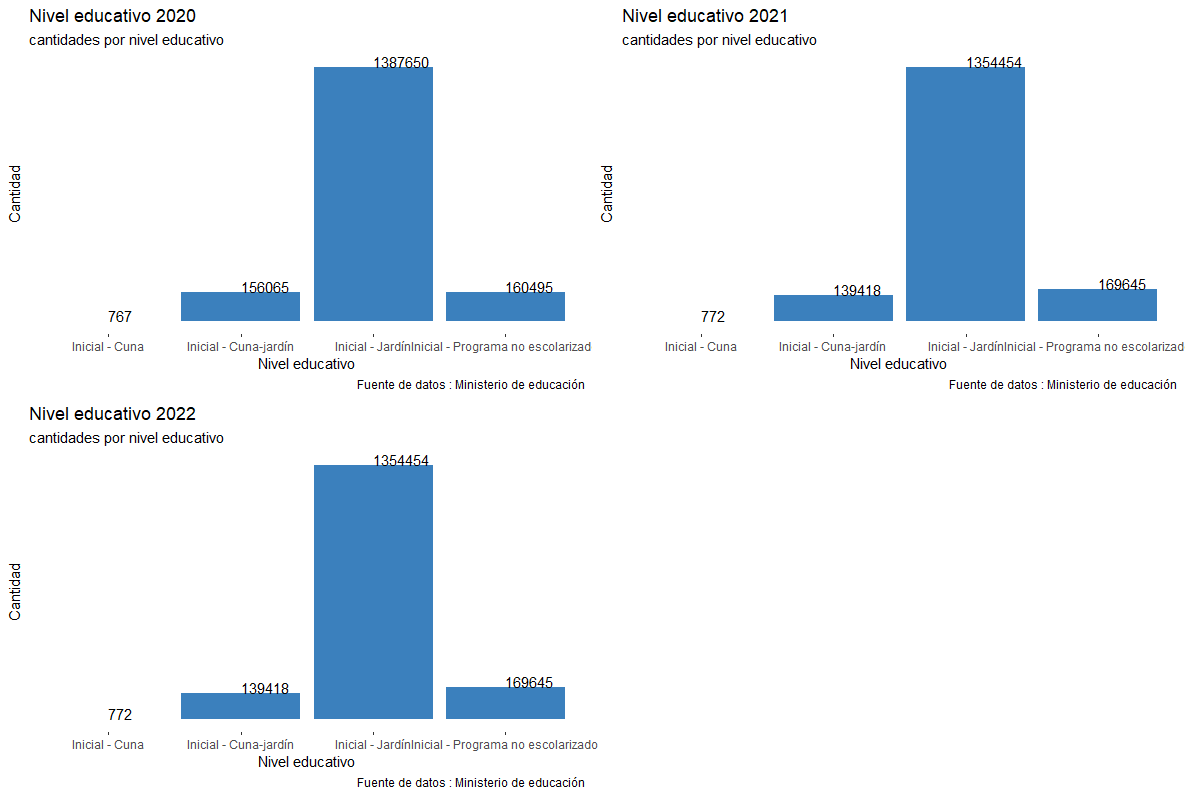
\includegraphics[width=1.2\textwidth]{Figures/nivelesEducativos}
\decoRule
\caption[Nivel Educativo]{Niveles educativos}
\label{fig:niveleseducativos}
\end{figure}

\section{Evolución mensual de matrículas}\label{res_evolucion_matriculas}

En este análisis se identificó la evolución que han tenido la cantidad de matrículas de cada mes en los últimos 3 años, las siguientes imágenes~\ref{fig:matriculas} muestran la evolución por año.\\
Se aprecia una mayor cantidad de incidencias entre Marzo y Abril, esto se puede entender por el inicio del año escolar en el Perú. Y en menor medida hay una cantidad elevada de matrículas desde el inicio de año, durante el resto del año se ve una menor cantidad pero si ocurren, esto podría deberse posiblemente a traslados de colegio.

\begin{figure}[h]
\centering
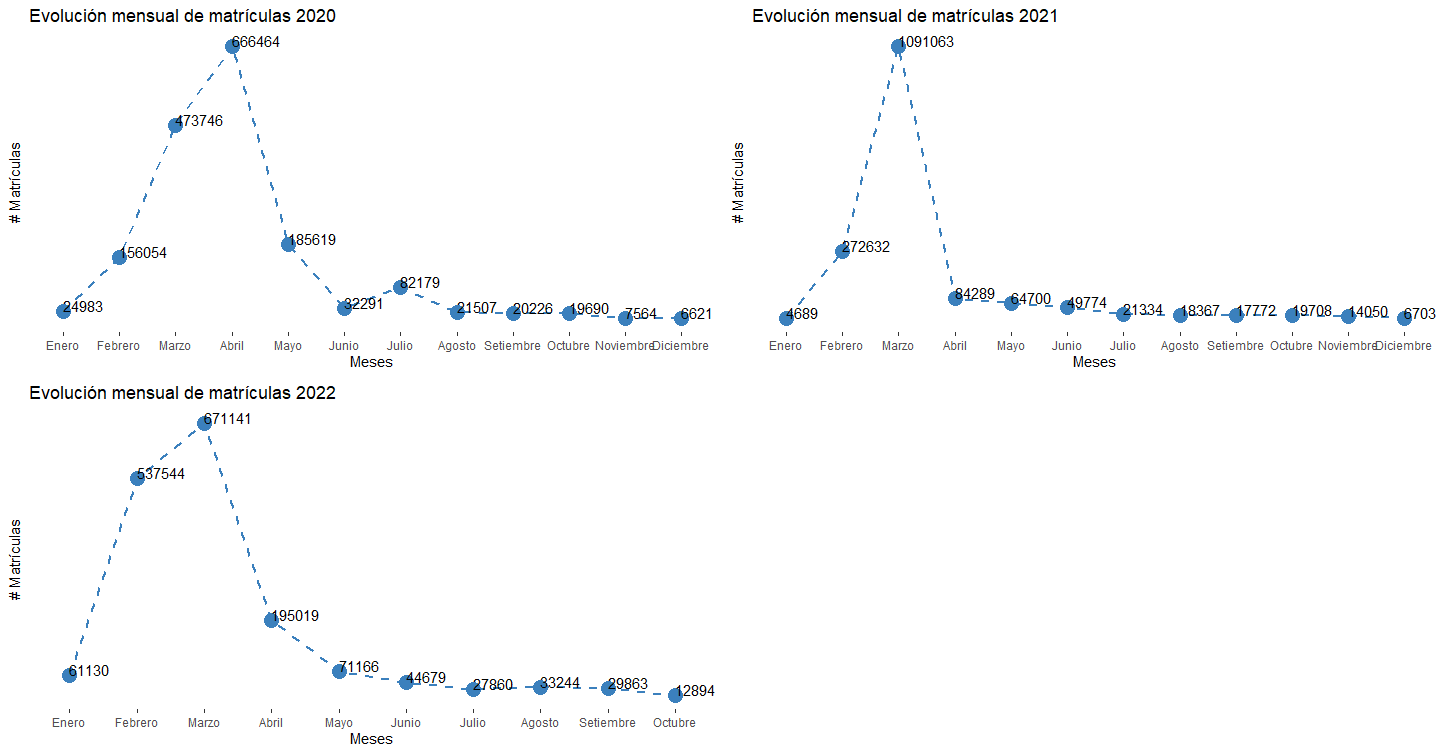
\includegraphics[width=1.2\textwidth]{Figures/evolucionMatriculas}
\decoRule
\caption[Matrículas]{Evolución de cantidades por cada mes}
\label{fig:matriculas}
\end{figure}

\section{Discapacidad}

El presente gráfico~\ref{fig:discapacidad} queremos mostrar la cantidad de estudiantes con alguna discapacidad sea visual, sordoceguera, autismo, auditiva entre otros.\\
Se puede apreciar que en los últimos 2 años se tenía mayor incidencia en las discapacidades motora, intelectual y autismo, pero en el presente año han disminuído las que tienen que ver con motora e intelectual, pero el autismo se mantiene como un factor predominante.

\begin{figure}[th]
\centering
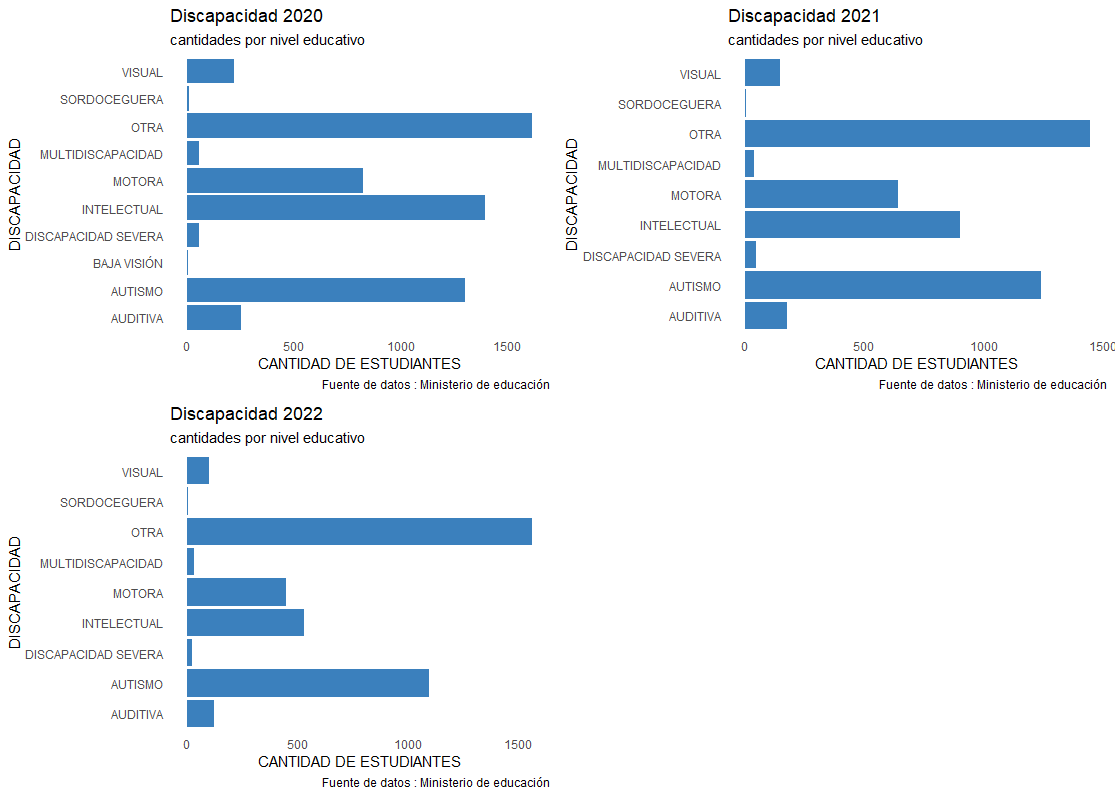
\includegraphics[width=0.8\textwidth]{Figures/discapacidad}
\decoRule
\caption[Discapacidad]{Tipos de discapacidad}
\label{fig:discapacidad}
\end{figure}


\section{Nacionalidad de estudiantes}

Se muestra a continuación una imagen~\ref{fig:nacionalidad} la distribución de nacionalidades, teniendo como mayor cantidad, luego de la peruana, la nacionalidad Venezolana, debido a que hay muchos países en este análisis, se ve conveniente el uso de una tabla para poder mostrar los datos.

\begin{figure}[!h]
\centering
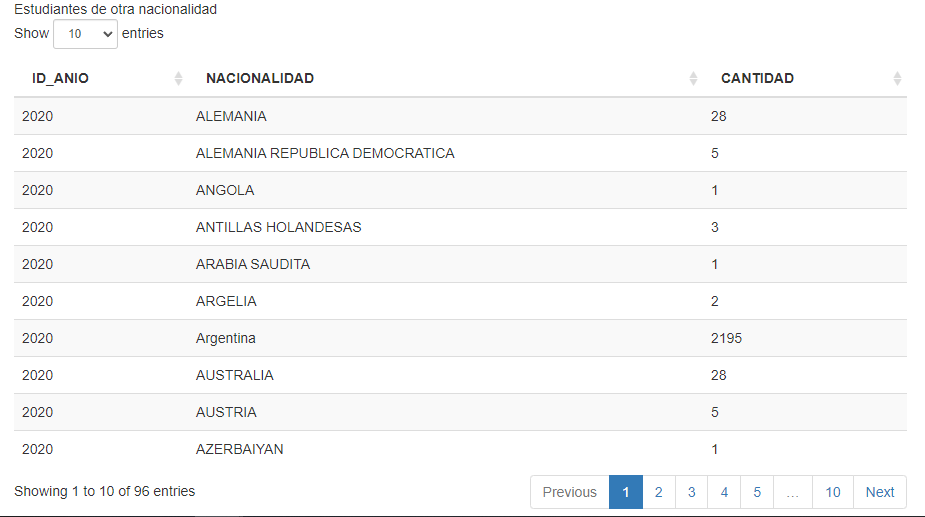
\includegraphics[width=1\textwidth]{Figures/nacionalidad}
\decoRule
\caption[Nacionalidad]{Nacionalidad de estudiantes}
\label{fig:nacionalidad}
\end{figure}

\section{Distribución de género}

En la imagen~\ref{fig:genero} se pueden apreciar distribuciones simulares entre hombres y mujeres.

\begin{figure}[!h]
\centering
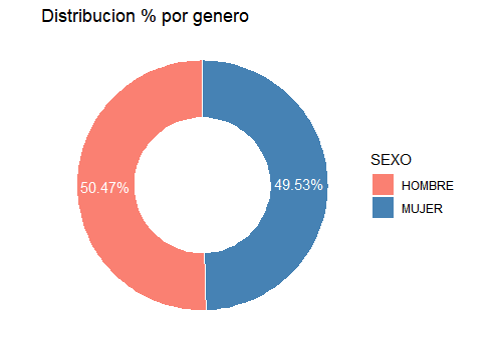
\includegraphics[width=0.8\textwidth]{Figures/genero}
\decoRule
\caption[Genero]{Distribuciones de género}
\label{fig:genero}
\end{figure}

\section{DNI Validados}

En la imagen~\ref{fig:validaciondni} se aprecia que hay una gran mayoría de documentos validados, pero se ve en menor medida estudiantes indocumentados.

\begin{figure}[!h]
\centering
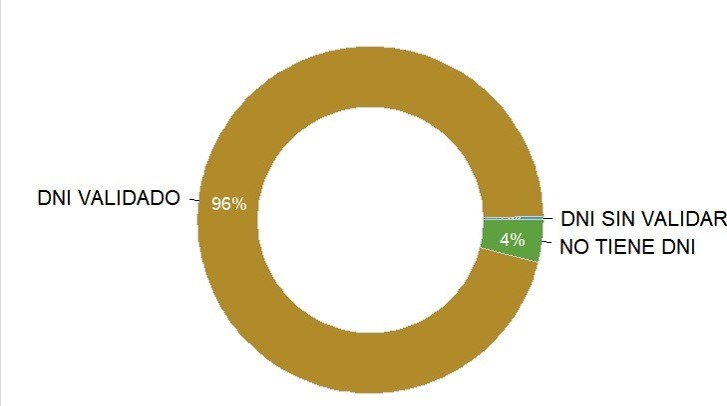
\includegraphics[width=0.8\textwidth]{Figures/validacionDNI}
\decoRule
\caption[DNI Validados]{Validaciones de DNI}
\label{fig:validaciondni}
\end{figure}

\section{Representación por Shiny}
En shiny se desarrolló un panel que tiene un filtro por año para poder filtrar los gráficos presentados anteriormente según la imagen~\ref{fig:shiny}, la reactividad ante este campo de entrada permite tener la visualización de lo que ocurre por año.
\begin{figure}[th]
\centering
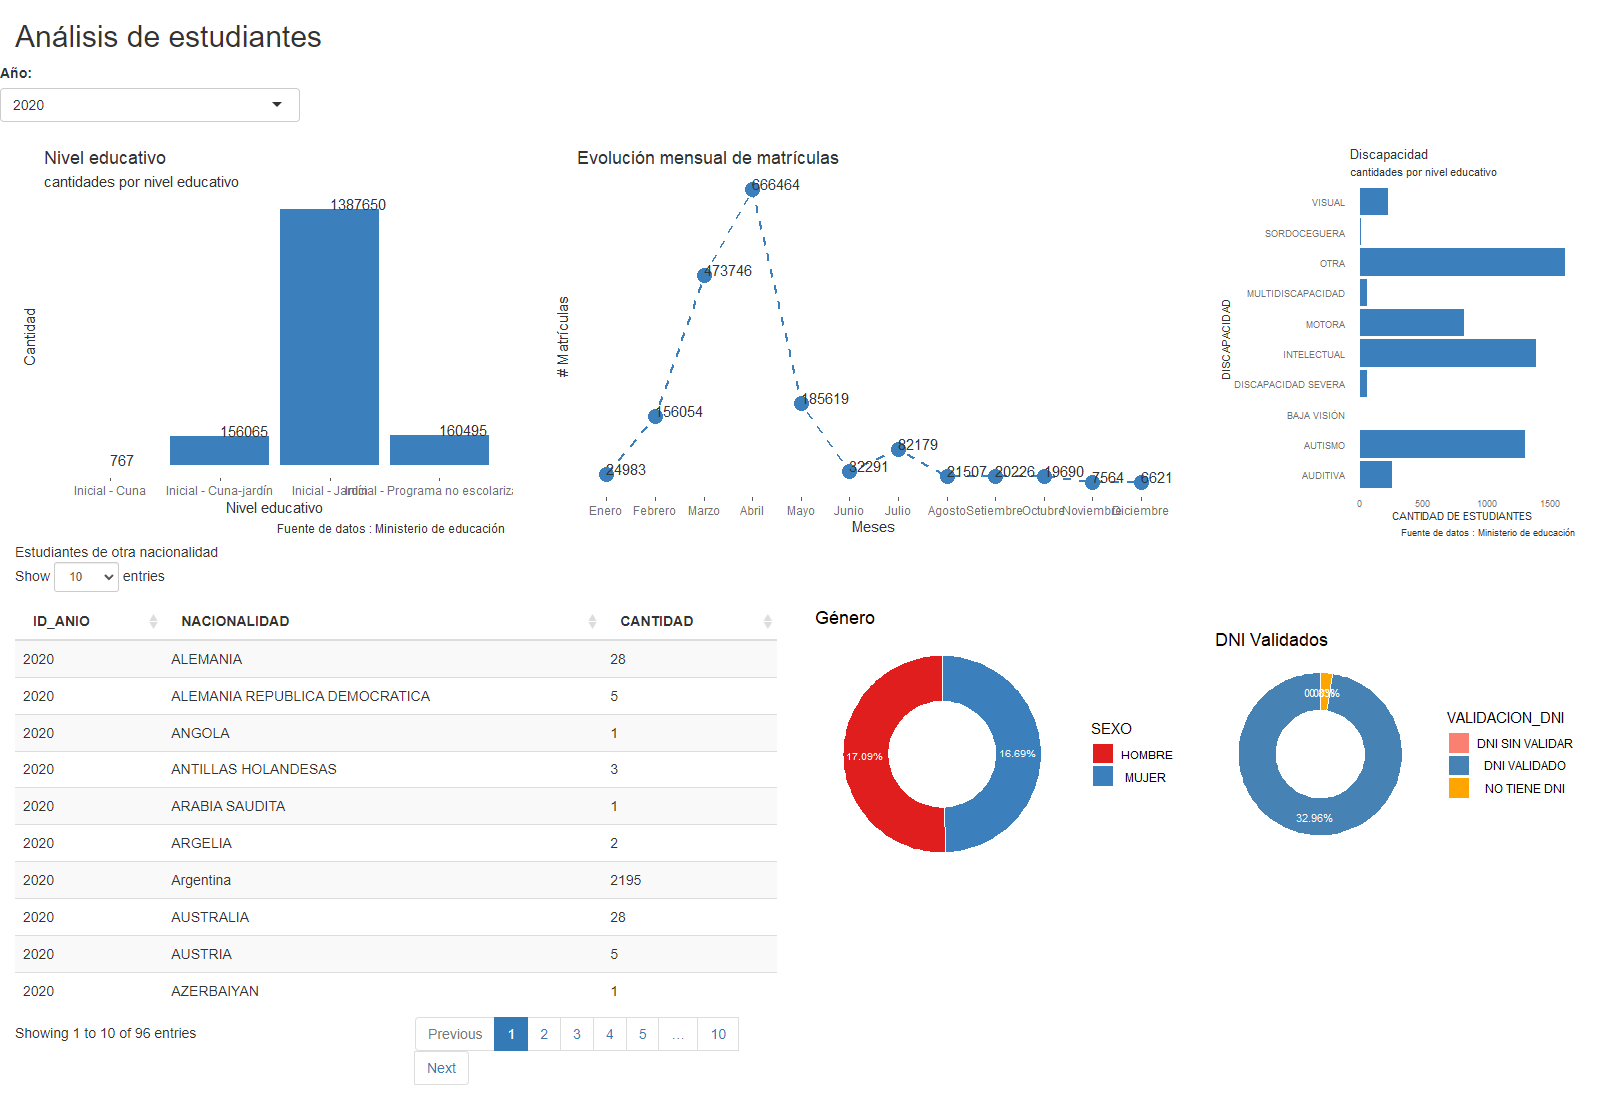
\includegraphics[width=1\textwidth]{Figures/shiny}
\decoRule
\caption[Shiny]{Representación mediante Shiny}
\label{fig:shiny}
\end{figure}

\section{Representaciones de ubicación de instituciones educativas por mapa}

Ya que es importante conocer la ubicación de los colegios, se realizó un mapa utilizando las librerias ggplot2, tidyverse y mapview en R, esta última librería proporciona funciones para crear visualizaciones interactivas de datos espaciales de manera muy rápida y conveniente. El código de estas representaciones se encuentra en el anexo \ref{cod_mapas}

Diagrama~\ref{fig:mapa1}: Su objetivo principal es llenar el vacío del trazado interactivo rápido (sin grado de presentación) para examinar e investigar visualmente ambos aspectos de los datos espaciales, las geometrías y sus atributos

\begin{figure}[th]
\centering
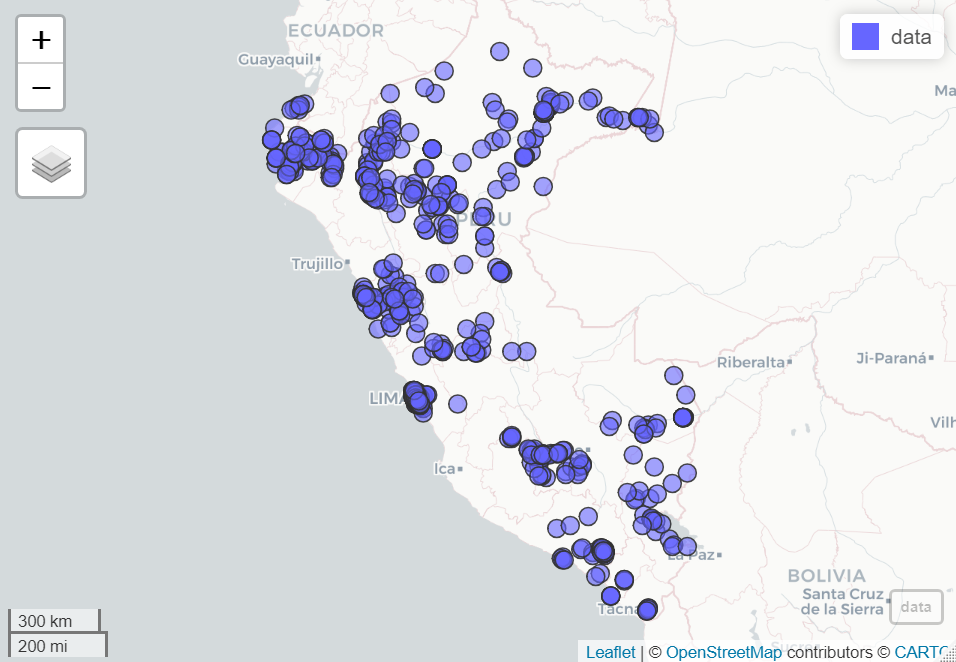
\includegraphics[width=1\textwidth]{Figures/mapa1}
\decoRule
\caption[Mapa]{Representación geográfica}
\label{fig:mapa1}
\end{figure}

Diagrama~\ref{fig:mapa2}: También podemos ver un conteo rápido del número de colegios por sector, con la librería leaflet, con una muestra que se extrajo, podemos ver a medida que vamos aumentando el zoom en que zonas entan mayor concentrados los colegios. 

\begin{figure}[th]
\centering
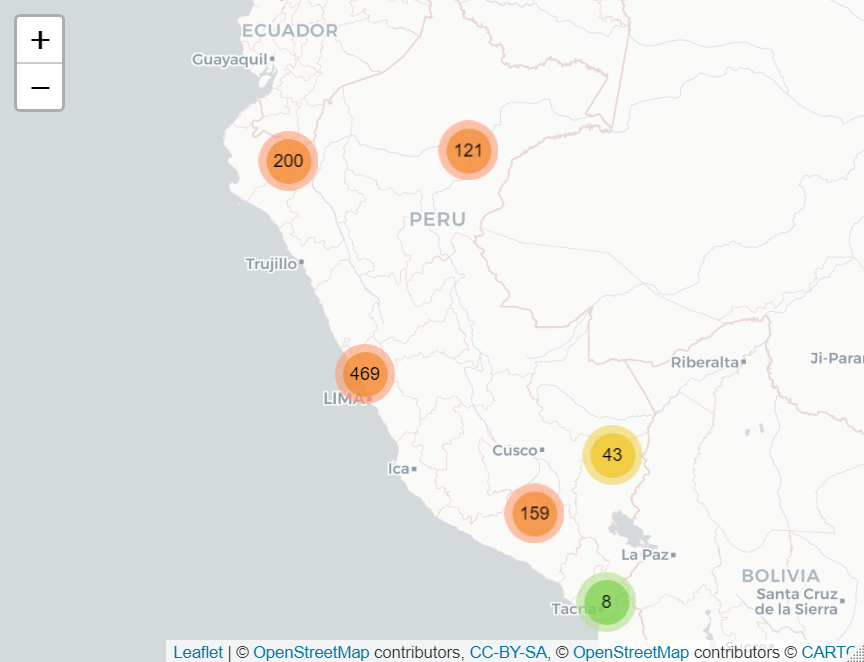
\includegraphics[width=1\textwidth]{Figures/mapa2}
\decoRule
\caption[Mapa]{Colegios}
\label{fig:mapa2}
\end{figure}

Diagrama~\ref{fig:mapa3}:Aprovechamos la interactividad del gráfico y cada que acercamos (zoom) nos muestra la cantidad de colegios acumulados en cada zona.

\begin{figure}[th]
\centering
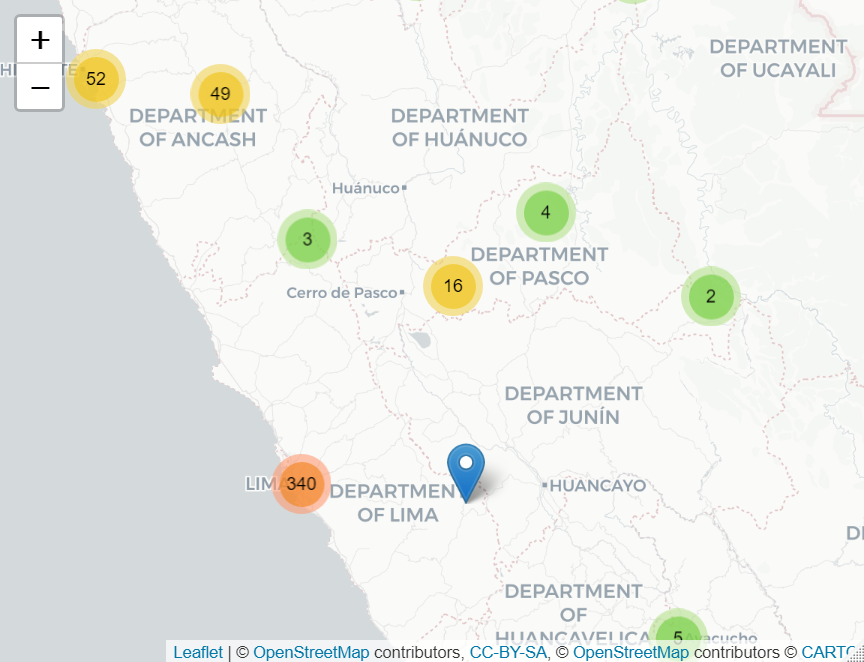
\includegraphics[width=1\textwidth]{Figures/mapa3}
\decoRule
\caption[Mapa]{Instituciones educativas acumuladas}
\label{fig:mapa3}
\end{figure}
%\include{Chapters/Chapter4} 
%\include{Chapters/Chapter5} 


%----------------------------------------------------------------------------------------
% THESIS CONTENT - APPENDICES
%----------------------------------------------------------------------------------------
\appendix % Cue to tell LaTeX that the following "chapters" are Appendices

% Include the appendices of the thesis as separate files from the Appendices folder
% Uncomment the lines as you write the Appendices
%\include{Appendices/AppendixA}
% from https://www.zhaw.ch/en/lsfm/study/studiweb/master-ls/masters-thesis/
%\include{Appendices/AppendixB}
%\include{Appendices/AppendixC}
%\include{Appendices/DeclarationOfOriginalityZHAW} 


%----------------------------------------------------------------------------------------
% BIBLIOGRAPHY
%----------------------------------------------------------------------------------------
\printbibliography[heading=bibintoc, title=Bibliografía]

%----------------------------------------------------------------------------------------

\end{document}  
